\documentclass{beamer}
\usetheme{Singapore}
\usepackage[utf8]{inputenc}
\usecolortheme{crane}
\usepackage{graphicx}
\usepackage{iwona}
\usepackage{hyperref}
\usepackage[ruled]{algorithm2e}
\usepackage{listings}

\lstset{language=Python,
basicstyle=\ttfamily\bfseries,
commentstyle=\color{red}\itshape,
stringstyle=\color{darkgreen},
showstringspaces=false,
keywordstyle=\color{blue}\bfseries}

\beamertemplatenavigationsymbolsempty

% defining styles for tikz
\usepackage{tikz}
\usetikzlibrary{shapes.geometric, arrows}
\tikzstyle{process} = [rectangle, minimum width=2cm, minimum height=1.5cm, text centered, text width=2.2cm, draw=black, fill=orange!80]
\tikzstyle{decision} = [diamond, minimum width=2cm, minimum height=1.5cm, text centered, text width=2.2cm, draw=black, fill=green!80]
\tikzstyle{arrow} = [thick,->,>=stealth]

\tikzstyle{boardclass} = [rectangle, minimum width=3.6cm, text width=3.6cm,minimum height=3.5cm, draw=black, fill=cyan!50]
\tikzstyle{squareclass} = [rectangle, minimum width=3.6cm, text width=3.6cm, minimum height=2cm, draw=black, fill=orange!50]
\tikzstyle{robotclass} = [rectangle, minimum width=3.6cm, minimum height=7.1cm, text width=3.6cm, draw=black, fill=green!50]
\tikzstyle{codebox} = [rectangle, minimum width = 2cm, draw=none, fill=none]
\tikzstyle{chooseaction} = [rectangle, minimum width=10cm, minimum height=1.2cm, draw=red, ultra thick, fill=none]
\tikzstyle{learning} = [rectangle, minimum width=10.5cm, minimum height=1cm, draw=red, ultra thick, fill=none]
\tikzstyle{movement} = [rectangle, minimum width=6cm, minimum height=0.4cm, draw=red, ultra thick, fill=none]
\tikzstyle{reset} = [rectangle, minimum width=10cm, minimum height=1.4cm, draw=red, ultra thick, fill=none]
\tikzstyle{stt} = [rectangle, draw=none, fill=none]

\tikzstyle{Arrow} = [->, shorten >=1pt, thick]
\tikzstyle{words} = [rectangle, text width=1.5cm, draw=none, fill=none]
\tikzstyle{dates} = [rectangle, draw=none, fill=none]





\setbeamerfont{caption}{size=\tiny}


\title
{I Wrote My First Line of Code $1\frac{1}{4}$ Years Ago}
\author{Geraint Palmer}
\date{}


\begin{document}
\frame{\titlepage}

% 1st slide, journey to code (vba to python)
\begin{frame}
  \frametitle{My Journey to Code}
	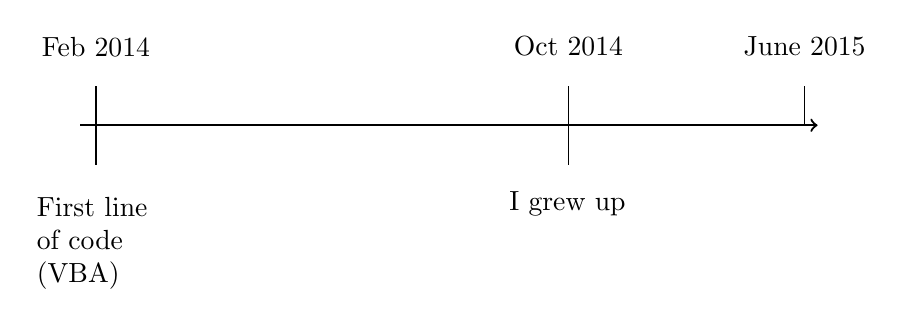
\begin{tikzpicture}
		\draw [Arrow] (-0.2, 0) -- (9.2, 0);
		\draw (0, 0) -- (0, 0.5);
		\node (feb2014) [dates, yshift=1cm] {Feb 2014};
		\draw (9, 0) -- (9, 0.5);
		\node (June2015) [dates, yshift=1cm, xshift=9cm] {June 2015};
		\draw(0, 0) -- (0, -0.5);
		\node (firstlineofcode) [words, yshift=-1.5cm] {First line of code (VBA)};
		\pause
		\draw (6, 0) -- (6, 0.5);
		\node (oct2014) [dates, yshift=1cm, xshift=6cm] {Oct 2014};
		\draw (6, 0) -- (6, -0.5);
		\node (python) [words, yshift=-1cm, xshift=6cm] {I grew up};
	\end{tikzpicture}
\end{frame}

% 2nd slide, journey to code (python to now)
\begin{frame}
  \frametitle{My Journey to Code}
	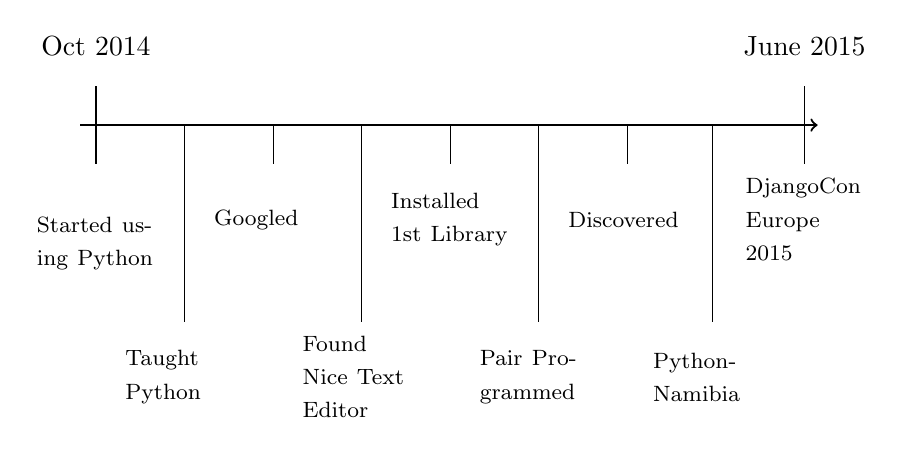
\begin{tikzpicture}
		\draw [Arrow] (-0.2, 0) -- (9.2, 0);
		\draw (0, 0) -- (0, 0.5);
		\node (oct2014) [dates, yshift=1cm] {Oct 2014};
		\draw (9, 0) -- (9, 0.5);
		\node (June2015) [dates, yshift=1cm, xshift=9cm] {June 2015};
		\draw(0, 0) -- (0, -0.5);
		\node (python) [words, yshift=-1.5cm] {\footnotesize{Started using Python}};
		\pause
		\draw (1.125, 0) -- (1.125, -2.5);
		\node (python) [words, yshift=-3.2cm, xshift=1.125cm] {\footnotesize{Taught Python}};
		\pause
		\draw (2.25, 0) -- (2.25, -0.5);
		\node (python) [words, yshift=-1.2cm, xshift=2.25cm] {\footnotesize{Googled}};
		\pause
    \draw (3.375, 0) -- (3.375, -2.5);
    \node (python) [words, yshift=-3.2cm, xshift=3.375cm] {\footnotesize{Found Nice Text Editor}};
    \pause
		\draw (4.5, 0) -- (4.5, -0.5);
		\node (python) [words, yshift=-1.2cm, xshift=4.5cm] {\footnotesize{Installed 1st Library}};
		\pause
		\draw (5.625, 0) -- (5.625, -2.5);
		\node (python) [words, yshift=-3.2cm, xshift=5.625cm] {\footnotesize{Pair Programmed}};
		\pause
		\draw (6.75, 0) -- (6.75, -0.5);
		\node (python) [words, yshift=-1.2cm, xshift=6.75cm] {\footnotesize{Discovered}};
		\pause
		\draw (7.825, 0) -- (7.825, -2.5);
		\node (python) [words, yshift=-3.2cm, xshift=7.825cm] {\footnotesize{Python-Namibia}};
    \pause
    \draw (9.0, 0) -- (9.0, -0.5);
    \node (python) [words, yshift=-1.2cm, xshift=9cm] {\footnotesize{DjangoCon Europe 2015}};
	\end{tikzpicture}
\end{frame}


\end{document}